% section1_introduction.tex — Module A: Yue
\section{Introduction}\label{sec:introduction}

\subsection{Background}

Bike-sharing systems have become an integral component of urban transportation infrastructure, providing flexible, environmentally friendly mobility options. Understanding the factors that drive daily rental demand is critical for operational planning and resource allocation.

\subsection{Dataset}

We use the UCI Bike Sharing Dataset \citep{fanaee2014}, which records daily aggregated rental counts from the Capital Bikeshare system in Washington, D.C., spanning 731 days (2011--2012). The dataset includes meteorological covariates, calendar indicators, and rental counts.

\textbf{Important note on normalisation:} The variables \texttt{temp} and \texttt{hum} in the original dataset are already normalised. Specifically, $\texttt{temp} = (T + 8) / 47$ where $T \in [-8, 39]$\textdegree C, and $\texttt{hum} = \text{humidity} / 100$. Consequently, regression coefficients represent the change in daily rentals per unit change in the \emph{normalised} scale, not raw physical units. Care must be taken when interpreting effect sizes.

\subsection{Subsampling Strategy}

To facilitate the sequential updating extension (Extension B), we subsample $n = 360$ observations from the full dataset using a fixed random seed (\texttt{random\_state = 42}). This yields four equal blocks of 90 observations each, ordered chronologically, enabling demonstration of how posterior beliefs evolve as data accumulates.

\subsection{Exploratory Overview}

% TODO: update file paths once figures are finalised
Figure~\ref{fig:cnt_hist} shows the distribution of daily rental counts in the subsampled data.

\begin{figure}[htbp]
    \centering
    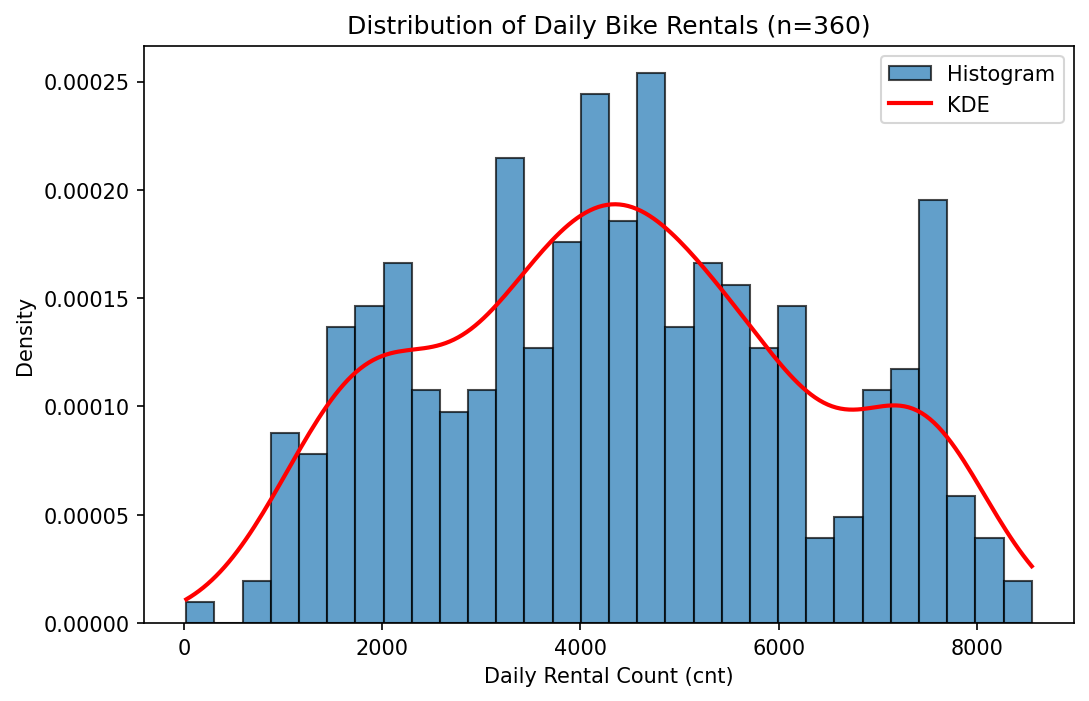
\includegraphics[width=0.7\textwidth]{../results/figures/cnt_histogram.png}
    \caption{Distribution of daily bike rentals ($n=360$). The distribution is approximately symmetric and unimodal, supporting the use of a Normal likelihood.}
    \label{fig:cnt_hist}
\end{figure}

Figure~\ref{fig:corr_heatmap} presents the correlation structure among numeric variables.

\begin{figure}[htbp]
    \centering
    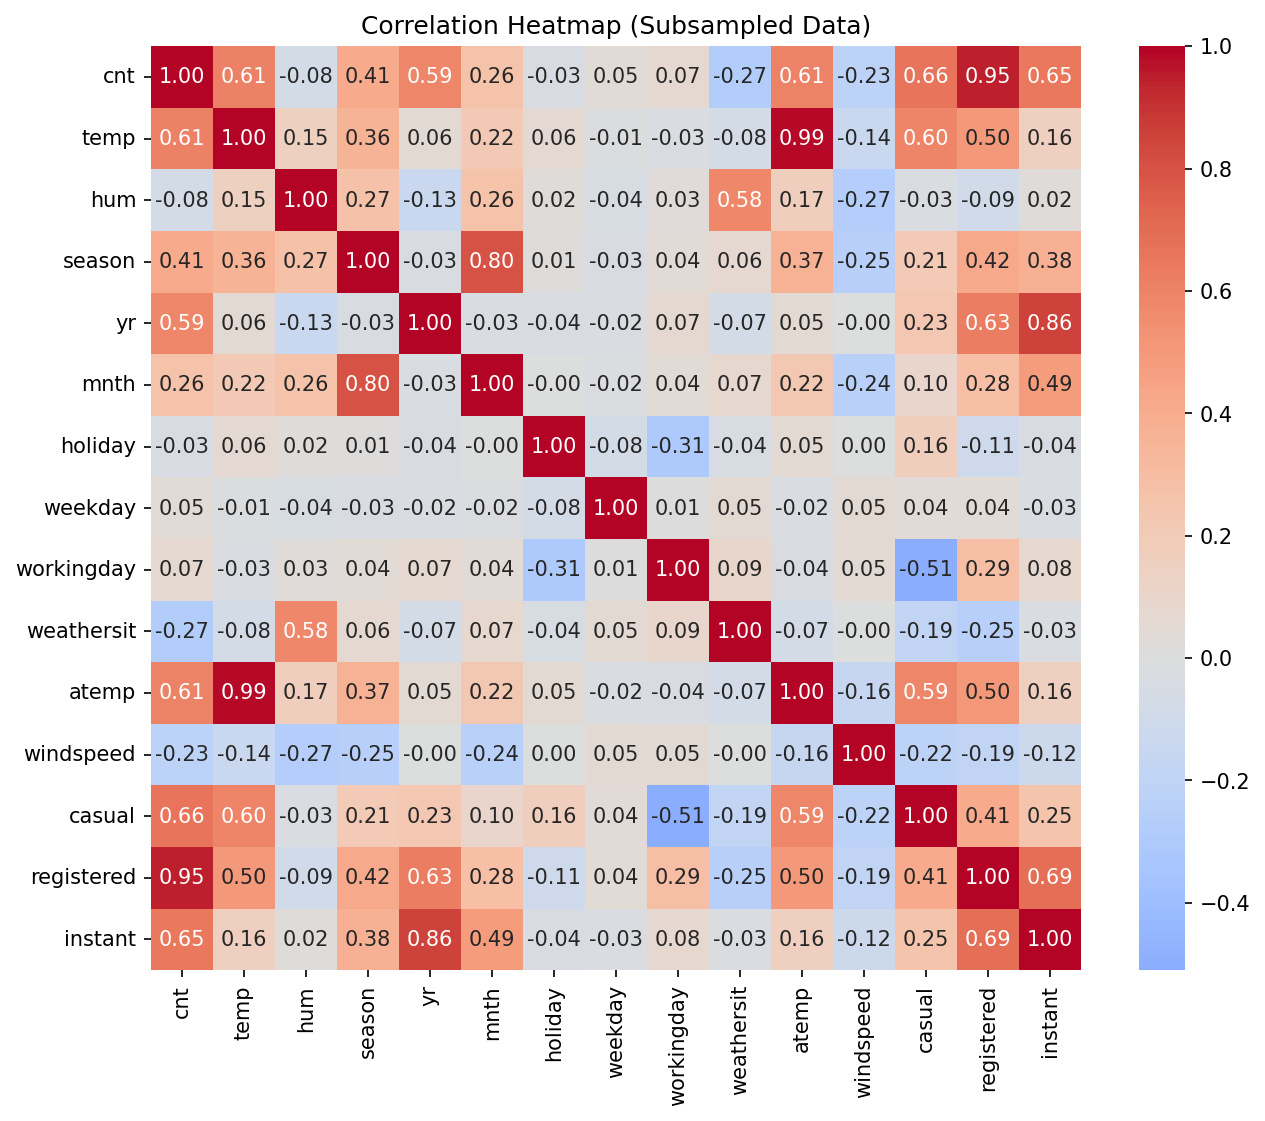
\includegraphics[width=0.8\textwidth]{../results/figures/correlation_heatmap.png}
    \caption{Correlation heatmap of numeric variables in the subsampled dataset.}
    \label{fig:corr_heatmap}
\end{figure}

\subsection{Research Objectives}

This report aims to:
\begin{enumerate}
    \item Specify and justify a likelihood function for daily rental counts (Section~\ref{sec:likelihood});
    \item Develop a Bayesian linear regression model with informative priors;
    \item Compare Bayesian posterior inference with frequentist maximum likelihood estimates (Section~\ref{sec:frequentist});
    \item Demonstrate sequential updating and conduct sensitivity analyses.
\end{enumerate}
